% !TEX TS-program = xelatex
% !TEX encoding = UTF-8 Unicode

\documentclass[AutoFakeBold]{LZUThesis}
\usepackage{wasysym}
\usepackage{enumitem}
\usepackage[most]{tcolorbox}
\usepackage{multirow}
\usepackage{tikz}
\usetikzlibrary{arrows.meta, decorations.markings}
\usepackage{hyperref}
\usepackage[numbers,sort&compress]{natbib}
\newcommand{\upcite}[1]{\textsuperscript{\textsuperscript{\cite{#1}}}}
\allowdisplaybreaks[4]

% for verilog code coloring
\definecolor{vgreen}{RGB}{104,180,104}
\definecolor{vblue}{RGB}{49,49,255}
\definecolor{vorange}{RGB}{255,143,102}

\lstdefinestyle{verilog-style}
{
    language=Verilog,
    basicstyle=\small\ttfamily,
    keywordstyle=\color{vblue},
    identifierstyle=\color{black},
    commentstyle=\color{vgreen},
    numbers=left,
    numberstyle=\tiny\color{black},
    numbersep=10pt,
    tabsize=8,
    moredelim=*[s][\colorIndex]{[}{]},
    literate=*{:}{:}1
}

\makeatletter
\newcommand*\@lbracket{[}
\newcommand*\@rbracket{]}
\newcommand*\@colon{:}
\newcommand*\colorIndex{%
    \edef\@temp{\the\lst@token}%
    \ifx\@temp\@lbracket \color{black}%
    \else\ifx\@temp\@rbracket \color{black}%
    \else\ifx\@temp\@colon \color{black}%
    \else \color{vorange}%
    \fi\fi\fi
}
\makeatother

\usepackage{trace}

\begin{document}

\title{{实验四 ALU模块实现}}

\entitle{Experiment 4 ALU Module Implementation}

\author{生物信息学班 李泽华 320210928501}
\major{计算机组成原理}
\advisor{高平}
\college{生命科学学院}
\grade{2021级}


\frontmatter

% \ZhAbstract{
% }{
% }

%\EnAbstract{
%}{
%}

%\customcontent

\mainmatter

% \chapter{\texorpdfstring{绪 \quad 论}{绪论}}
\chapter{实验目的}
\begin{enumerate}
    \item 熟悉 MIPS 指令集中的运算指令,学会对这些指令进行归纳分类。
    \item 了解 MIPS 指令结构。
    \item 熟悉并掌握 ALU 的原理、功能和设计。
    \item 进一步加强运用 verilog 语言进行电路设计的能力。
    \item 为后续设计 cpu 的实验打下基础。
\end{enumerate}

\chapter{实验任务与要求}
\section{试验任务}
\begin{enumerate}
    \item 学习 MIPS 指令集,熟知指令类型,了解指令功能和编码,归纳基础的 ALU 运算指令。
    \item 归纳确定自己本次实验中准备实现的 ALU 运算,要求不实现定点乘除指令和浮点运算指令,要求至少实现 5 种 ALU 运算,其中要包含加减运算,其中减法在内部要转换为加法,与加法运算共同调用实验一里自己完成的加法模块去做。
    \item 自行设计本次实验的方案,画出结构框图,大致结构框图如图 5.1。图 5.1 中的操作码位数和类型请自行设计,可以设计为独热码(一位有效编码)或二进制编码。比如,设计方案中预定实现 7 种 ALU 运算,则操作码采用独热码,则需 7bit 数据,每位单独指示一种运算;若采用二进制编码,则只用 3bit 数据位即可,但在需ALU 内部先进行解码,才能确定 ALU 作何种运算。
    \item 根据设计的实验方案,使用 verilog 编写相应代码。
    \item 对编写的代码进行仿真,得到正确的波形图。
    \item 将以上设计作为一个单独的模块,设计一个外围模块去调用该模块, 外围模块中需调用封装好的 LCD 触摸屏模块,显示 ALU 的两个源操作数、操作码和运算结果,并且需要利用触摸功能输入源操作数。操作码可以考虑用 LCD 触摸屏输入,也可以用拨码开关输入。
    \item 将编写的代码进行综合布局布线,并下载到试验箱中的 FPGA 板子上进行演示。
\end{enumerate}
\section{实验要求}
\begin{enumerate}
    \item 实验箱结果截图(可按小组截图)
    \item 代码注释(单独注释,着重说明16位所涉及的地方)
\end{enumerate}

\chapter{实验结果}
\section{实验代码}
\subsection{加法器}
\begin{lstlisting}[style=verilog-style]
module adder(
    input  [31:0] operand1, // 32位输入
    input  [31:0] operand2, // 32位输入
    input         cin,      // 进位
    output [31:0] result,   // 32位输出
    output        cout      // 进位输出
    );
    assign {cout,result} = operand1 + operand2 + cin;

endmodule
\end{lstlisting}

\subsection{ALU}
\begin{lstlisting}[style=verilog-style]
module alu(
    input  [11:0] alu_control,  // ALU控制信号
    input  [31:0] alu_src1,     // ALU操作数1,为补码
    input  [31:0] alu_src2,     // ALU操作数2,为补码
    output [31:0] alu_result    // ALU结果
    );

    // ALU控制信号,独热码
    wire alu_add;   //加法操作
    wire alu_sub;   //减法操作
    wire alu_slt;   //有符号比较,小于置位,复用加法器做减法
    wire alu_sltu;  //无符号比较,小于置位,复用加法器做减法
    wire alu_and;   //按位与
    wire alu_nor;   //按位或非
    wire alu_or;    //按位或
    wire alu_xor;   //按位异或
    wire alu_sll;   //逻辑左移
    wire alu_srl;   //逻辑右移
    wire alu_sra;   //算术右移
    wire alu_lui;   //高位加载

    assign alu_add  = alu_control[11];
    assign alu_sub  = alu_control[10];
    assign alu_slt  = alu_control[ 9];
    assign alu_sltu = alu_control[ 8];
    assign alu_and  = alu_control[ 7];
    assign alu_nor  = alu_control[ 6];
    assign alu_or   = alu_control[ 5];
    assign alu_xor  = alu_control[ 4];
    assign alu_sll  = alu_control[ 3];
    assign alu_srl  = alu_control[ 2];
    assign alu_sra  = alu_control[ 1];
    assign alu_lui  = alu_control[ 0];

    wire [31:0] add_sub_result;
    wire [31:0] slt_result;
    wire [31:0] sltu_result;
    wire [31:0] and_result;
    wire [31:0] nor_result;
    wire [31:0] or_result;
    wire [31:0] xor_result;
    wire [31:0] sll_result;
    wire [31:0] srl_result;
    wire [31:0] sra_result;
    wire [31:0] lui_result;

    assign and_result = alu_src1 & alu_src2;      // 与结果为两数按位与
    assign or_result  = alu_src1 | alu_src2;      // 或结果为两数按位或
    assign nor_result = ~or_result;               // 或非结果为或结果按位取反
    assign xor_result = alu_src1 ^ alu_src2;      // 异或结果为两数按位异或
    assign lui_result = {alu_src2[15:0], 16'd0};  // 立即数装载结果为立即数移位至高半字节

//-----{加法器}begin
//add,sub,slt,sltu均使用该模块
    wire [31:0] adder_operand1;
    wire [31:0] adder_operand2;
    wire        adder_cin     ;
    wire [31:0] adder_result  ;
    wire        adder_cout    ;
    assign adder_operand1 = alu_src1; 
    assign adder_operand2 = alu_add ? alu_src2 : ~alu_src2; 
    assign adder_cin      = ~alu_add; //减法需要cin 
    adder adder_module(
    .operand1(adder_operand1),
    .operand2(adder_operand2),
    .cin     (adder_cin     ),
    .result  (adder_result  ),
    .cout    (adder_cout    )
    );

    //加减结果
    assign add_sub_result = adder_result;

    //slt结果
    //adder_src1[31] adder_src2[31] adder_result[31]
    //       0             1           X(0或1)       "正-负",显然小于不成立
    //       0             0             1           相减为负,说明小于
    //       0             0             0           相减为正,说明不小于
    //       1             1             1           相减为负,说明小于
    //       1             1             0           相减为正,说明不小于
    //       1             0           X(0或1)       "负-正",显然小于成立
    assign slt_result[31:1] = 31'd0;
    assign slt_result[0]    = (alu_src1[31] & ~alu_src2[31]) | (~(alu_src1[31]^alu_src2[31]) & adder_result[31]);

    //sltu结果
    //对于32位无符号数比较,相当于33位有符号数({1'b0,src1}和{1'b0,src2})的比较,最高位0为符号位
    //故,可以用33位加法器来比较大小,需要对{1'b0,src2}取反,即需要{1'b0,src1}+{1'b1,~src2}+cin
    //但此处用的为32位加法器,只做了运算:                             src1   +    ~src2   +cin
    //32位加法的结果为{adder_cout,adder_result},则33位加法结果应该为{adder_cout+1'b1,adder_result}
    //对比slt结果注释,知道,此时判断大小属于第二三种情况,即源操作数1符号位为0,源操作数2符号位为0
    //结果的符号位为1,说明小于,即adder_cout+1'b1为2'b01,即adder_cout为0
    assign sltu_result = {31'd0, ~adder_cout};
//-----{加法器}end

//-----{移位器}begin
    // 移位分三步进行,
    // 第一步根据移位量低2位即[1:0]位做第一次移位,
    // 第二步在第一次移位基础上根据移位量[3:2]位做第二次移位,
    // 第三步在第二次移位基础上根据移位量[4]位做第三次移位。
    wire [4:0] shf;
    assign shf = alu_src1[4:0];
    wire [1:0] shf_1_0;
    wire [1:0] shf_3_2;
    assign shf_1_0 = shf[1:0];
    assign shf_3_2 = shf[3:2];
    
     // 逻辑左移
    wire [31:0] sll_step1;
    wire [31:0] sll_step2;
    assign sll_step1 = {32{shf_1_0 == 2'b00}} & alu_src2                   // 若shf[1:0]="00",不移位
                     | {32{shf_1_0 == 2'b01}} & {alu_src2[30:0], 1'd0}     // 若shf[1:0]="01",左移1位
                     | {32{shf_1_0 == 2'b10}} & {alu_src2[29:0], 2'd0}     // 若shf[1:0]="10",左移2位
                     | {32{shf_1_0 == 2'b11}} & {alu_src2[28:0], 3'd0};    // 若shf[1:0]="11",左移3位
    assign sll_step2 = {32{shf_3_2 == 2'b00}} & sll_step1                  // 若shf[3:2]="00",不移位
                     | {32{shf_3_2 == 2'b01}} & {sll_step1[27:0], 4'd0}    // 若shf[3:2]="01",第一次移位结果左移4位
                     | {32{shf_3_2 == 2'b10}} & {sll_step1[23:0], 8'd0}    // 若shf[3:2]="10",第一次移位结果左移8位
                     | {32{shf_3_2 == 2'b11}} & {sll_step1[19:0], 12'd0};  // 若shf[3:2]="11",第一次移位结果左移12位
    assign sll_result = shf[4] ? {sll_step2[15:0], 16'd0} : sll_step2;     // 若shf[4]="1",第二次移位结果左移16位

    // 逻辑右移
    wire [31:0] srl_step1;
    wire [31:0] srl_step2;
    assign srl_step1 = {32{shf_1_0 == 2'b00}} & alu_src2                   // 若shf[1:0]="00",不移位
                     | {32{shf_1_0 == 2'b01}} & {1'd0, alu_src2[31:1]}     // 若shf[1:0]="01",右移1位,高位补0
                     | {32{shf_1_0 == 2'b10}} & {2'd0, alu_src2[31:2]}     // 若shf[1:0]="10",右移2位,高位补0
                     | {32{shf_1_0 == 2'b11}} & {3'd0, alu_src2[31:3]};    // 若shf[1:0]="11",右移3位,高位补0
    assign srl_step2 = {32{shf_3_2 == 2'b00}} & srl_step1                  // 若shf[3:2]="00",不移位
                     | {32{shf_3_2 == 2'b01}} & {4'd0, srl_step1[31:4]}    // 若shf[3:2]="01",第一次移位结果右移4位,高位补0
                     | {32{shf_3_2 == 2'b10}} & {8'd0, srl_step1[31:8]}    // 若shf[3:2]="10",第一次移位结果右移8位,高位补0
                     | {32{shf_3_2 == 2'b11}} & {12'd0, srl_step1[31:12]}; // 若shf[3:2]="11",第一次移位结果右移12位,高位补0
    assign srl_result = shf[4] ? {16'd0, srl_step2[31:16]} : srl_step2;    // 若shf[4]="1",第二次移位结果右移16位,高位补0
 
    // 算术右移
    wire [31:0] sra_step1;
    wire [31:0] sra_step2;
    assign sra_step1 = {32{shf_1_0 == 2'b00}} & alu_src2                                 // 若shf[1:0]="00",不移位
                     | {32{shf_1_0 == 2'b01}} & {alu_src2[31], alu_src2[31:1]}           // 若shf[1:0]="01",右移1位,高位补符号位
                     | {32{shf_1_0 == 2'b10}} & {{2{alu_src2[31]}}, alu_src2[31:2]}      // 若shf[1:0]="10",右移2位,高位补符号位
                     | {32{shf_1_0 == 2'b11}} & {{3{alu_src2[31]}}, alu_src2[31:3]};     // 若shf[1:0]="11",右移3位,高位补符号位
    assign sra_step2 = {32{shf_3_2 == 2'b00}} & sra_step1                                // 若shf[3:2]="00",不移位
                     | {32{shf_3_2 == 2'b01}} & {{4{sra_step1[31]}}, sra_step1[31:4]}    // 若shf[3:2]="01",第一次移位结果右移4位,高位补符号位
                     | {32{shf_3_2 == 2'b10}} & {{8{sra_step1[31]}}, sra_step1[31:8]}    // 若shf[3:2]="10",第一次移位结果右移8位,高位补符号位
                     | {32{shf_3_2 == 2'b11}} & {{12{sra_step1[31]}}, sra_step1[31:12]}; // 若shf[3:2]="11",第一次移位结果右移12位,高位补符号位
    assign sra_result = shf[4] ? {{16{sra_step2[31]}}, sra_step2[31:16]} : sra_step2;    // 若shf[4]="1",第二次移位结果右移16位,高位补符号位
//-----{移位器}end

    // 选择相应结果输出
    assign alu_result = (alu_add|alu_sub) ? add_sub_result[31:0] : 
                        alu_slt           ? slt_result :
                        alu_sltu          ? sltu_result :
                        alu_and           ? and_result :
                        alu_nor           ? nor_result :
                        alu_or            ? or_result  :
                        alu_xor           ? xor_result :
                        alu_sll           ? sll_result :
                        alu_srl           ? srl_result :
                        alu_sra           ? sra_result :
                        alu_lui           ? lui_result :
                        32'd0;
endmodule
\end{lstlisting}

\subsection{tb}
\begin{lstlisting}[style=verilog-style]
module tb;

    reg   [11:0] alu_control;
    reg   [31:0] alu_src1;   
    reg   [31:0] alu_src2;   
    wire  [31:0] alu_result; 
    alu alu_module(
        .alu_control(alu_control),
        .alu_src1   (alu_src1   ),
        .alu_src2   (alu_src2   ),
        .alu_result (alu_result )
    );

    initial begin
        //加法操作
        alu_control = 12'b1000_0000_0000;
        alu_src1 = 32'd1;
        alu_src2 = 32'hffffffff;

        //减法操作
        #5;
        alu_control = 12'b0100_0000_0000;
        alu_src1 = 32'd1;
        alu_src2 = 32'd2;
        
        //有符号比较
        #5;
        alu_control = 12'b0010_0000_0000;
        alu_src1 = 32'd1;
        alu_src2 = 32'd2;
        
        //无符号比较
        #5;
        alu_control = 12'b0001_0000_0000;
        alu_src1 = 32'd1;
        alu_src2 = 32'd2;
        
        //按位与
        #5;
        alu_control = 12'b0000_1000_0000;
        alu_src1 = 32'h12345678;
        alu_src2 = 32'hf0f0f0f0;
        
        //按位或非
        #5;
        alu_control = 12'b0000_0100_0000;
        alu_src1 = 32'he;
        alu_src2 = 32'd1;

        //按位或
        #5;
        alu_control = 12'b0000_0010_0000;
        alu_src1 = 32'he;
        alu_src2 = 32'd1;
        
        //按位异或
        #5;
        alu_control = 12'b0000_0001_0000;
        alu_src1 = 32'b1010;
        alu_src2 = 32'b0101;
        
        //逻辑左移
        #5;
        alu_control = 12'b0000_0000_1000;
        alu_src1 = 32'd4;
        alu_src2 = 32'hf;
        
        //逻辑右移
        #5;
        alu_control = 12'b0000_0000_0100;
        alu_src1 = 32'd4;
        alu_src2 = 32'hf0;

        //算术右移        
        #5;
        alu_control = 12'b0000_0000_0010;
        alu_src1 = 32'd4;
        alu_src2 = 32'hf0000000;

        //高位加载    
        #5;
        alu_control = 12'b0000_0000_0001;
        alu_src2 = 32'hbfc0;
    end
endmodule
\end{lstlisting}

\section{仿真波形}
\begin{figure}[htbp]
    \centering
    \hfill
    \subfloat[0\textasciitilde40ns]{
        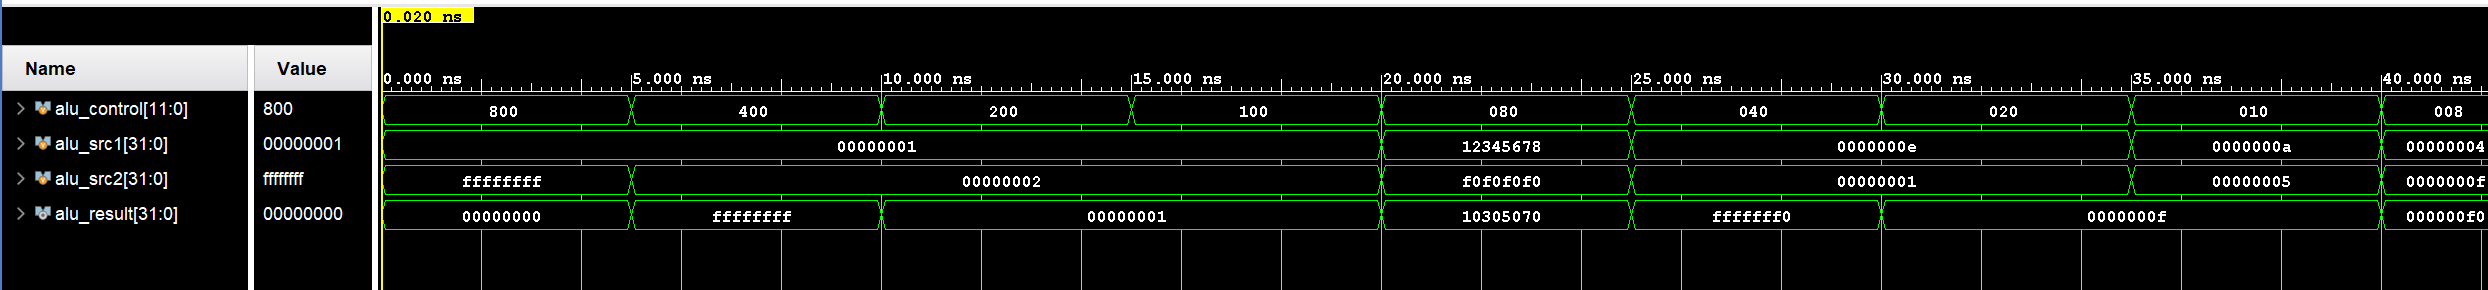
\includegraphics[width=0.45\textwidth]{img/wave_1}
    }
    \hfill
    \subfloat[40\textasciitilde58ns]{
        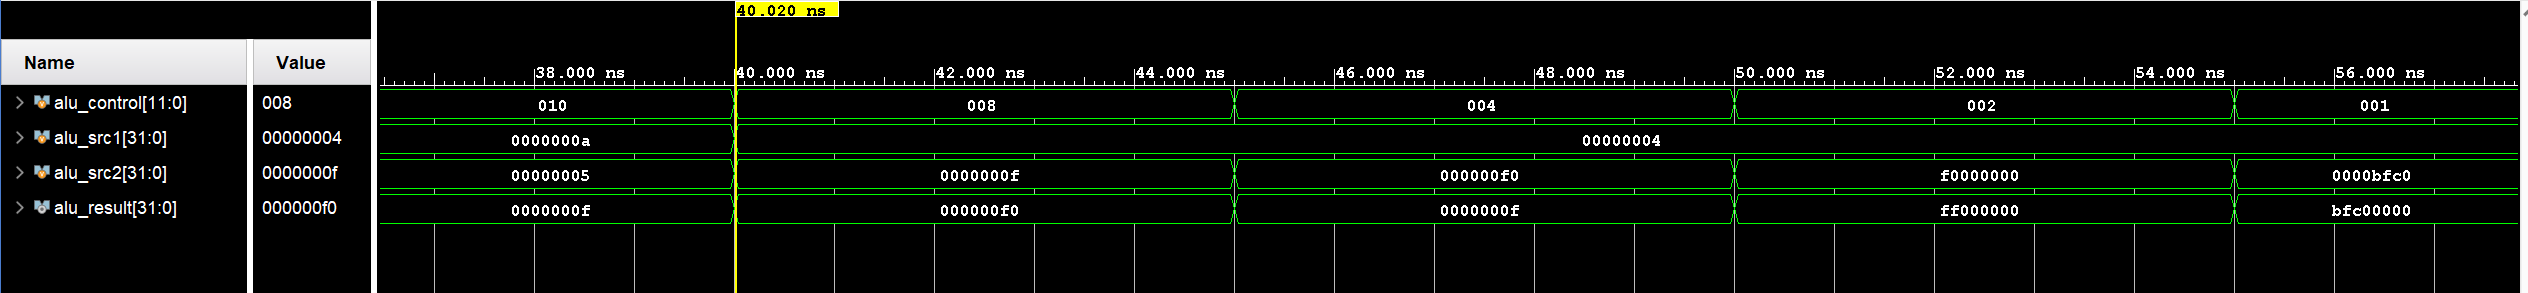
\includegraphics[width=0.45\textwidth]{img/wave_2}
    }
\end{figure}

\section{实验箱结果}
\begin{figure}[htbp]
    \centering
    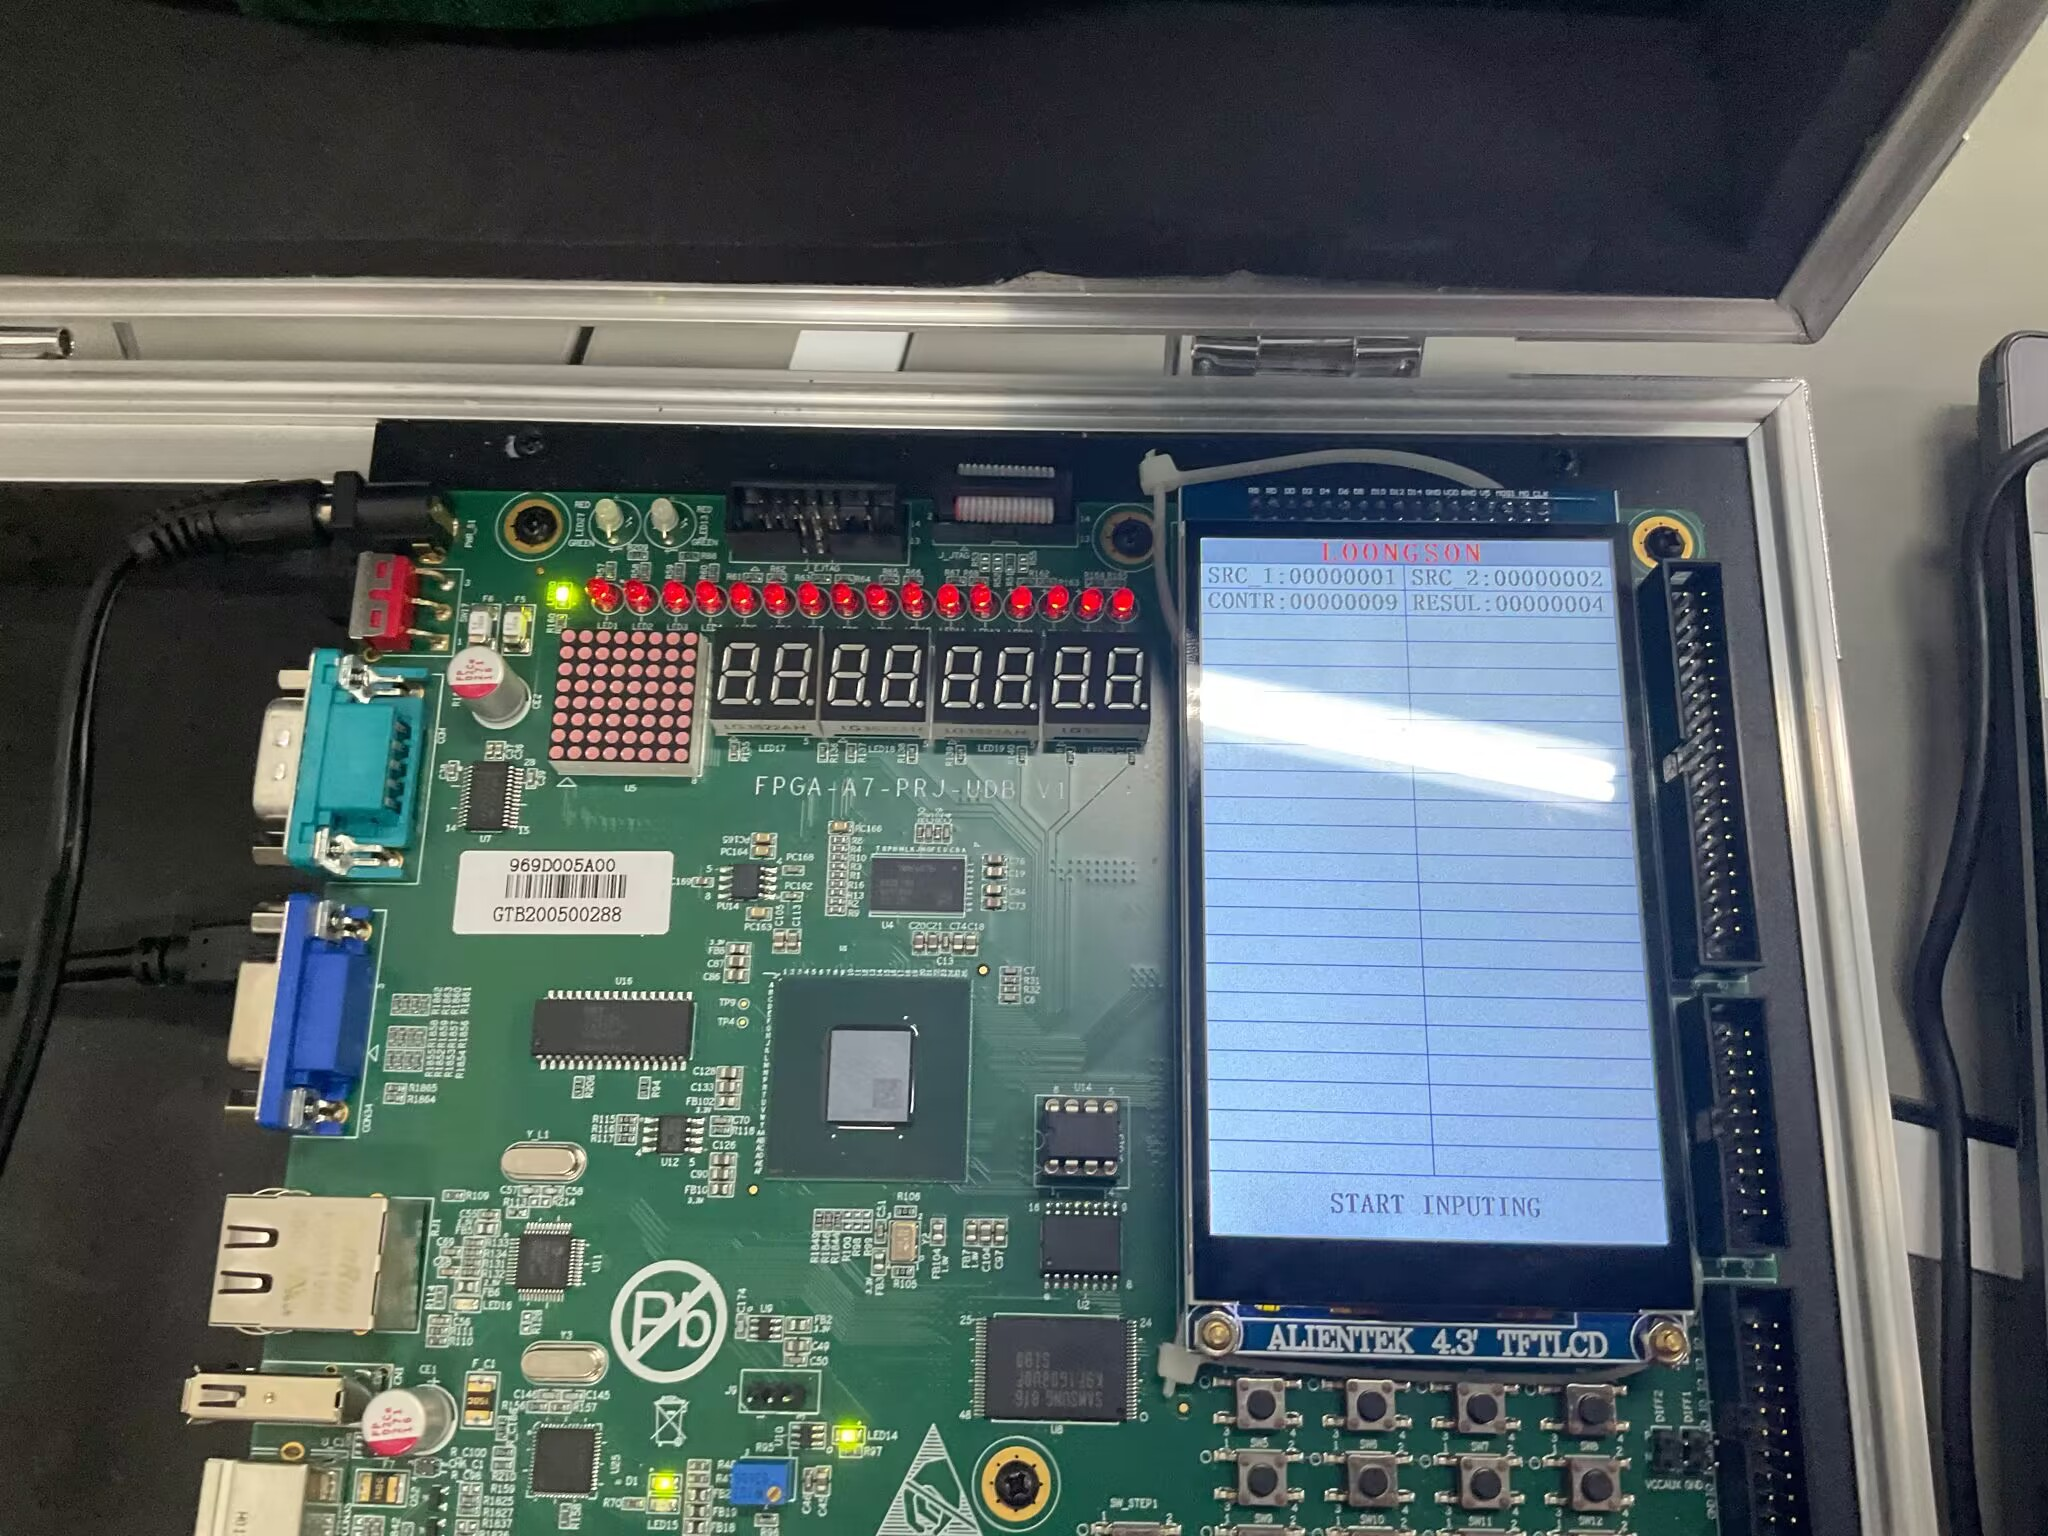
\includegraphics[width=0.8\textwidth]{img/result}
    \caption{实验箱结果(1<<2=4)}
\end{figure}

%\chapter{思考与讨论}

%\section{课后问题}
%论文后部
\backmatter


%=======%
%引入参考文献文件
%=======%
%\bibdatabase{bib/database}%bib文件名称 仅修改bib/ 后部分
%\printbib
%\nocite{*} %显示数据库中有的,但是正文没有引用的文献



\Appendix
参考链接:
\url{https://github.com/zehua0417/ComputerOrganizationAndArchitecture_exp}
\begin{figure}[htbp]
    \centering
    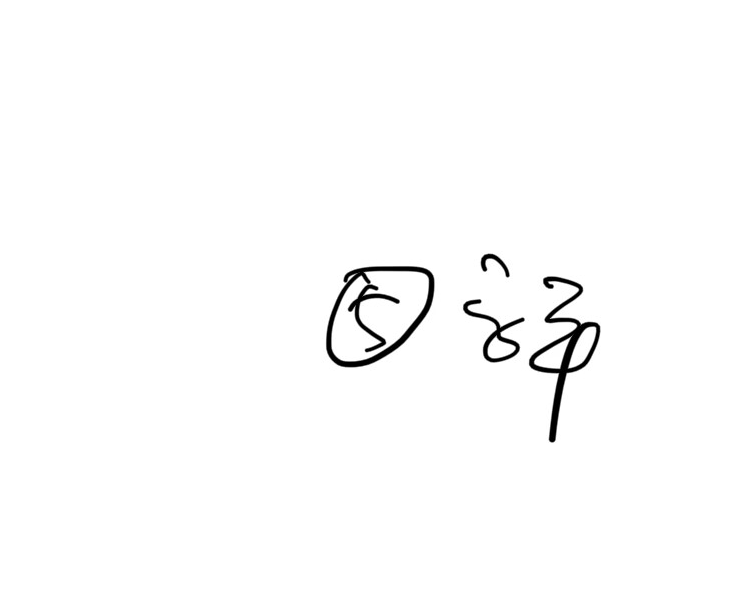
\includegraphics[width=0.4\textwidth]{img/sign}
\end{figure}

%\Thanks


%\Grade %这一句才是成绩页,上面是填写


\end{document}
